% Created 2026-06-04 Thu 09:23
% Intended LaTeX compiler: pdflatex
\documentclass[aspectratio=169,professionalfonts]{beamer}

\usepackage[utf8]{inputenc}
\usepackage[T1]{fontenc}
\usepackage{graphicx}
\usepackage{longtable}
\usepackage{wrapfig}
\usepackage{rotating}
\usepackage[normalem]{ulem}
\usepackage{amsmath}
\usepackage{amssymb}
\usepackage{capt-of}
\usepackage{hyperref}
\usepackage{booktabs}
\usepackage{amsmath,amssymb}
\usepackage{graphicx}
\setbeamertemplate{navigation symbols}{}
\setbeamertemplate{caption}[numbered]
\AtBeginSection[]{\begin{frame}<beamer>{Roadmap}\tableofcontents[currentsection]\end{frame}}
\usetheme{Madrid}
\usecolortheme{default}
\usefonttheme{professionalfonts}
\author{Binjian Xin}
\date{\today}
\title{Energy Optimization System of Electric Vehicles}
\subtitle{Real-world deep reinforcement learning for EV energy efficiency}
\hypersetup{
 pdfauthor={Binjian Xin},
 pdftitle={Energy Optimization System of Electric Vehicles},
 pdfkeywords={},
 pdfsubject={},
 pdfcreator={},
 pdflang={English}}
\begin{document}

\maketitle
\section*{Talk Map}
\label{sec:org79938a7}

\begin{frame}[label={sec:orgf491457}]{Thirty-minute structure}
\begin{center}
\begin{tabular}{rll}
Part & Topic & Time\\
\hline
1 & Problem and design principle & 5 min\\
2 & EOSEV formulation and system & 9 min\\
3 & Real-vehicle experiments & 12 min\\
4 & Discussion and deployment & 4 min\\
\end{tabular}
\end{center}
\end{frame}
\begin{frame}[label={sec:orgf67fe36}]{Main claim}
EOSEV improves battery electric vehicle energy efficiency by learning
bounded pedal-map updates from real driving data.

\begin{itemize}
\item Uses directly measurable signals: speed, accelerator, brake, voltage,
current
\item Keeps the driver and production VCU in the loop
\item Learns from measured energy consumption instead of shaped simulation
rewards
\item Shows about \(7\%\sim8\%\) weekly block-level energy reduction on a
public-road route
\end{itemize}
\end{frame}
\section*{Motivation}
\label{sec:org4594a55}

\begin{frame}[label={sec:org8cd0f66}]{Why energy optimization is still hard}
\begin{itemize}
\item Same vehicle and route can have different energy consumption
\item Longitudinal behavior dominates short-horizon energy demand
\item Real EV operation is noisy, partially observed, and non-repeatable
\item Simulation is incomplete for driver, traffic, road, and powertrain
details
\end{itemize}

\vspace{0.5em}

At \(50\,\mathrm{km/h}\), a representative \(2500\,\mathrm{kg}\) EV needs:

\begin{itemize}
\item About \(3.4\,\mathrm{kW}\) for rolling resistance
\item About \(1.0\,\mathrm{kW}\) for aerodynamic drag
\item About \(17.4\,\mathrm{kW}\) for \(0.5\,\mathrm{m/s^2}\) acceleration,
before drivetrain losses
\end{itemize}
\end{frame}
\begin{frame}[label={sec:orgf853691}]{Gap in existing DRL eco-driving work}
\begin{itemize}
\item Many studies rely on simulation, connected traffic assumptions, or
autonomous speed planning
\item Rewards often mix weighted fuel, electricity, comfort, and constraint
terms
\item Real-time deployment and hard production constraints are often
secondary
\item Generalization across routes, weather, and driving style remains weak
\end{itemize}

\vspace{0.5em}

EOSEV focuses on a narrower but production-relevant question:

\begin{quote}
Can an agent adapt the powertrain response using only signals already
available from the vehicle?
\end{quote}
\end{frame}
\section*{EOSEV Formulation}
\label{sec:orgf39bcd6}

\begin{frame}[label={sec:orgc749b66}]{Driver-in-the-loop control}
Without the agent, the driver controls speed through accelerator and
brake pedals, and the VCU maps pedal opening and speed to torque.

With EOSEV:

\begin{itemize}
\item The agent observes driver and vehicle signals
\item The agent outputs a bounded torque-map increment
\item The VCU remains the final authority for calibrated limits and safety
\end{itemize}

\vspace{0.8em}

\[
\Delta\tau = \pi_\theta(V, A, B)
\]
\end{frame}
\begin{frame}[label={sec:org80e1aac}]{Markov decision process}
\begin{center}
\begin{tabular}{ll}
Element & EOSEV design\\
\hline
State & \(s_t = (V_t, A_t, B_t)\)\\
Action & \(\Delta\tau_t\), bounded torque-request update\\
Reward & \(r_t = -U_t I_t T_s\)\\
Environment & Vehicle, road, traffic, and driver\\
Policy & Actor network used online\\
\end{tabular}
\end{center}

\vspace{0.5em}

Measured voltage and current make the reward directly tied to consumed
electric work.
\end{frame}
\begin{frame}[label={sec:org52c30e0}]{Action: modify the pedal map}
\begin{columns}
\begin{column}{0.48\columnwidth}
\begin{center}

\includegraphics[width=0.92\textwidth]{images/optimized/table_init.png}
\end{center}
\end{column}
\begin{column}{0.48\columnwidth}
\begin{center}

\includegraphics[width=0.92\textwidth]{images/optimized/table_final.png}
\end{center}
\end{column}
\end{columns}
\end{frame}
\begin{frame}[label={sec:org0717b75}]{Why this action is practical}
\begin{itemize}
\item Uses a production control interface: pedal map update
\item Supports range checks before deployment
\item Preserves torque, voltage, current, thermal, diagnostic, and
drivability safeguards
\item Allows fallback to nominal map if the model or data path fails
\item Keeps the driver in control of the vehicle
\end{itemize}
\end{frame}
\section*{Algorithm and System}
\label{sec:orgef8edeb}

\begin{frame}[label={sec:orge1dca4c}]{DDPG training loop}
EOSEV uses a customized Deep Deterministic Policy Gradient setup.

\begin{itemize}
\item Actor: maps state to bounded \(\Delta\tau\)
\item Critic: evaluates state-action pairs during training
\item Replay buffer: stores \((s_t, a_t, r_t, s'_t)\) records
\item Training: update actor and critic after each episode
\item Inference: actor only
\end{itemize}

\begin{center}

\includegraphics[width=0.38\textwidth]{images/optimized/ddpg-training.png}
\end{center}
\end{frame}
\begin{frame}[label={sec:orgc1f9303}]{Network role separation}
\begin{columns}
\begin{column}{0.52\columnwidth}
\begin{center}
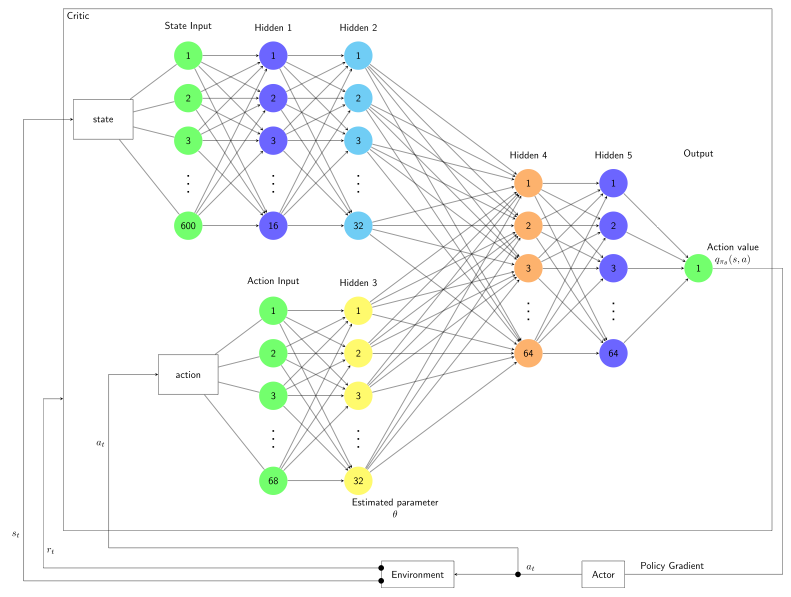
\includegraphics[width=\textwidth]{images/training.png}
\end{center}
\end{column}
\begin{column}{0.42\columnwidth}
\begin{center}
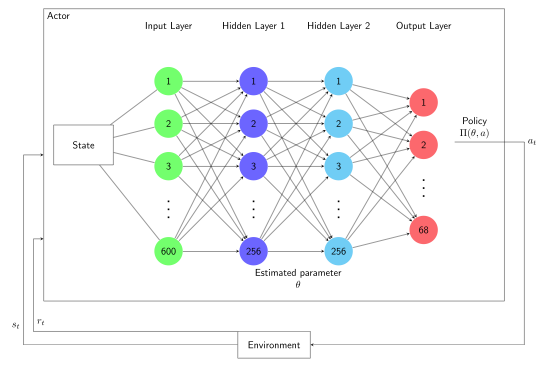
\includegraphics[width=\textwidth]{images/inference.png}
\end{center}
\end{column}
\end{columns}
\end{frame}
\begin{frame}[label={sec:orgee7ee46}]{Data record and replay buffer}
Each timestamped record stores an experience tuple:

\[
(t, s_t, a_t, r_t, s'_t)
\]

\[
s_t=(V_t,A_t,B_t), \quad r_t=-U_tI_tT_s
\]

\begin{itemize}
\item Sensor streams must be synchronized before training
\item Episodes provide a meaningful energy-consumption comparison unit
\item Low-density records are suitable for cloud upload and fleet-scale
offline learning
\end{itemize}
\end{frame}
\begin{frame}[label={sec:orgfb1be74}]{Deployment dataflow}
EOSEV supports cloud training, local training, and on-board inference.

\begin{itemize}
\item Scheduler configures dataflow states
\item Cruncher receives observations and forwards them to the Agent
\item Storage writes synchronized time-series records
\item Agent returns updated pedal maps or actor outputs
\item OTA can distribute validated model and map updates
\end{itemize}

\vspace{0.8em}

\begin{center}
\begin{tabular}{lllll}
Vehicle/ECU & -> & Cruncher & -> & Agent\\
Storage & <- & synchronized records & <- & Replay buffer\\
OTA update & <- & validated model/map & <- & Cloud training\\
\end{tabular}
\end{center}
\end{frame}
\section*{Experiments}
\label{sec:org3ec4b7f}

\begin{frame}[label={sec:orgb81984f}]{Proving-ground training setup}
\begin{itemize}
\item Fixed vehicle, driver, route, and speed profile
\item Vehicle accelerates from standstill to about \(17\,\mathrm{km/h}\) and
decelerates back to standstill
\item Episodes are discarded if speed remains outside the allowed band for
more than three seconds
\item Each three-hour run contains about 60 episodes
\item Training reloads previous model weights and pedal map
\end{itemize}

\begin{center}

\includegraphics[width=0.40\textwidth]{images/optimized/speed_profile.png}
\end{center}
\end{frame}
\begin{frame}[label={sec:org11d58f6}]{Driving-style monitoring}
Driving style is represented by the pedal-opening distribution.
\begin{columns}
\begin{column}{0.42\columnwidth}
\begin{center}

\includegraphics[width=\textwidth]{images/optimized/no-ai-driving-style.png}
\end{center}
\end{column}
\begin{column}{0.52\columnwidth}
\begin{center}

\includegraphics[width=\textwidth]{images/optimized/kld-c2.png}
\end{center}
\end{column}
\end{columns}
\end{frame}
\begin{frame}[label={sec:org6d83ca9}]{Proving-ground result}
\begin{itemize}
\item Energy consumption decreases within and across runs
\item Learned map requests larger negative torque at low speed and small
pedal opening
\item Regenerative braking is exploited implicitly through reward-driven
map updates
\end{itemize}

\begin{center}

\includegraphics[width=0.55\textwidth]{images/optimized/ddpg-training.png}
\end{center}
\end{frame}
\begin{frame}[label={sec:orga64c9d1}]{Public-road route 1}
\begin{columns}
\begin{column}{0.44\columnwidth}
\begin{center}
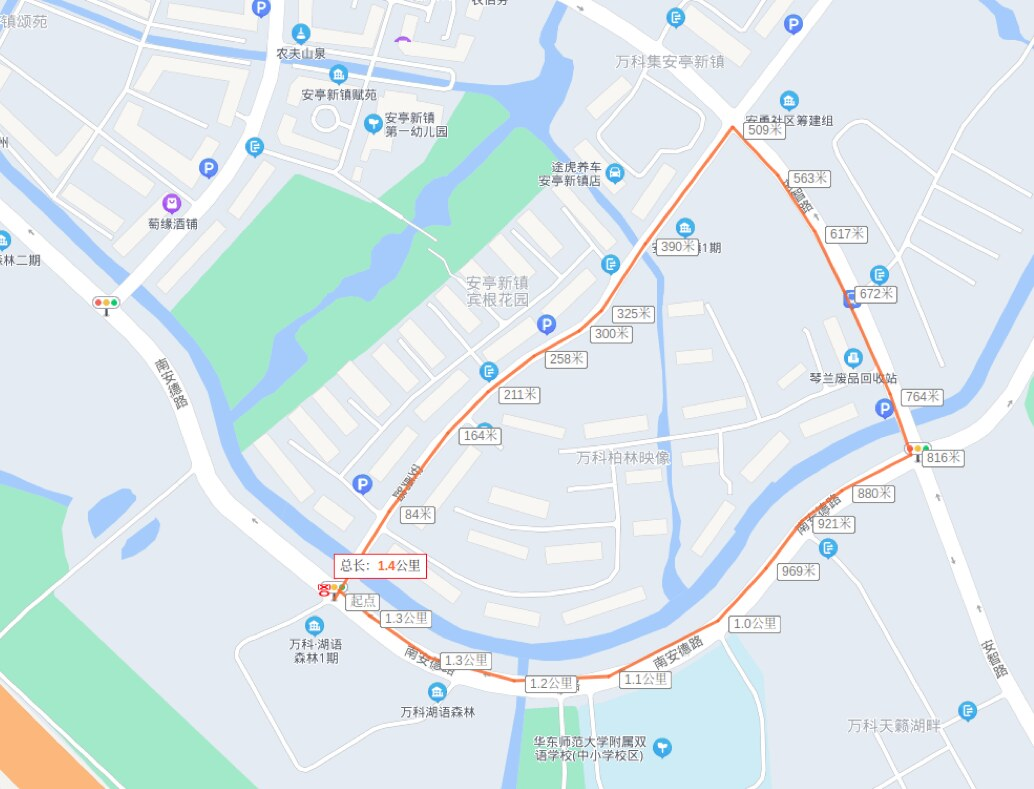
\includegraphics[width=\textwidth]{images/optimized/openroad_a_map.jpg}
\end{center}
\end{column}
\begin{column}{0.52\columnwidth}
\begin{center}
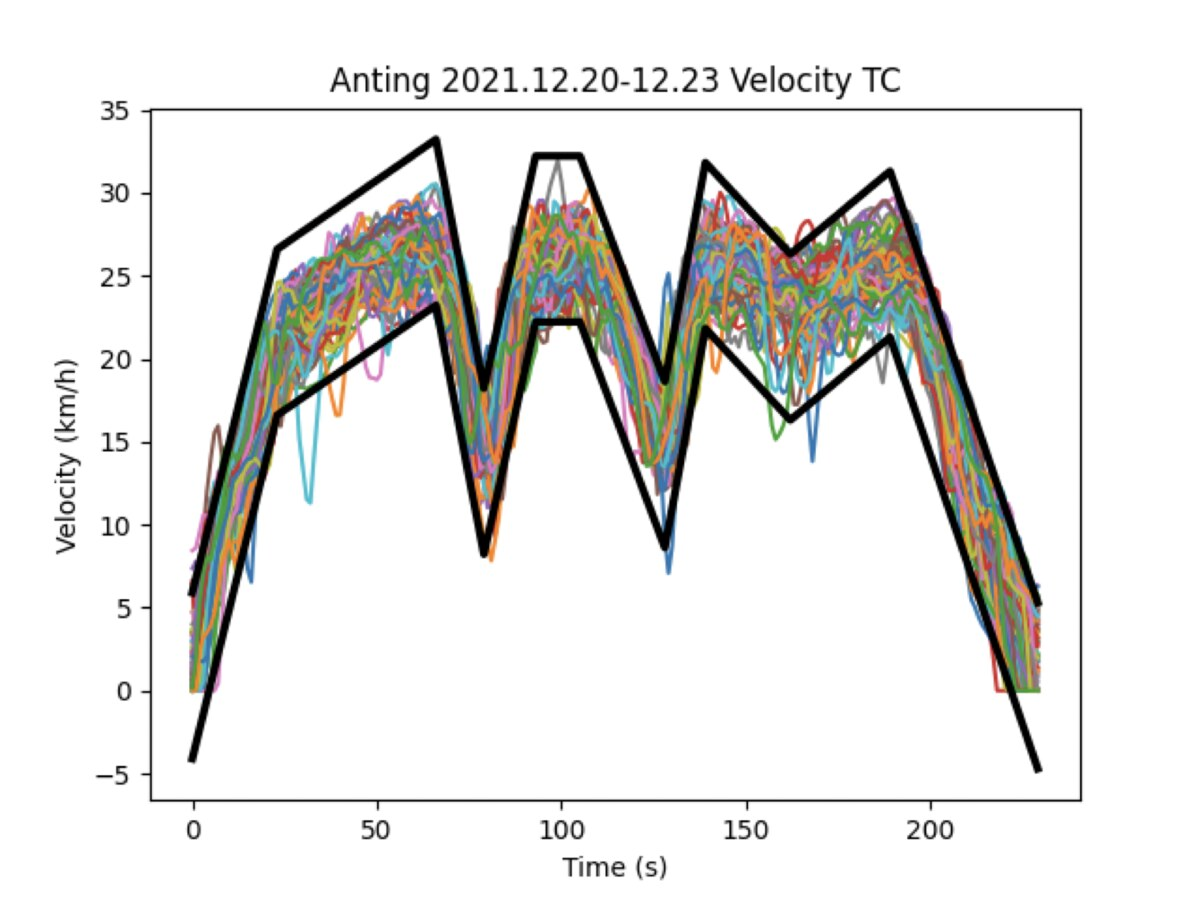
\includegraphics[width=\textwidth]{images/optimized/openroad_a_velocity.jpg}
\end{center}
\end{column}
\end{columns}
\end{frame}
\begin{frame}[label={sec:org187d3e4}]{Public-road route 1 result}
\begin{columns}
\begin{column}{0.52\columnwidth}
\begin{center}

\includegraphics[width=\textwidth]{images/optimized/openroad_a_consumption.png}
\end{center}
\end{column}
\begin{column}{0.42\columnwidth}
\begin{itemize}
\item Week 1: 8.16\% reduction
\item Week 2: 7.56\% reduction
\item Week 3: 7.03\% reduction
\item Mean: \(7.58\%\pm0.57\%\)
\end{itemize}
\end{column}
\end{columns}
\end{frame}
\begin{frame}[label={sec:orgfc2d28e}]{Route 1 driving-style drift}
The public-road run spans about 600 episodes, so style drift becomes
visible.

\begin{center}

\includegraphics[width=0.38\textwidth]{images/optimized/openroad_a_style.png}
\end{center}

\begin{itemize}
\item Longer tests require drift monitoring
\item Online training can adapt to changing driver behavior
\item Comparing same-week baselines helps control for weather and battery
heating effects
\end{itemize}
\end{frame}
\begin{frame}[label={sec:org6f62933}]{Transfer to route 2}
\begin{columns}
\begin{column}{0.52\columnwidth}
\begin{center}
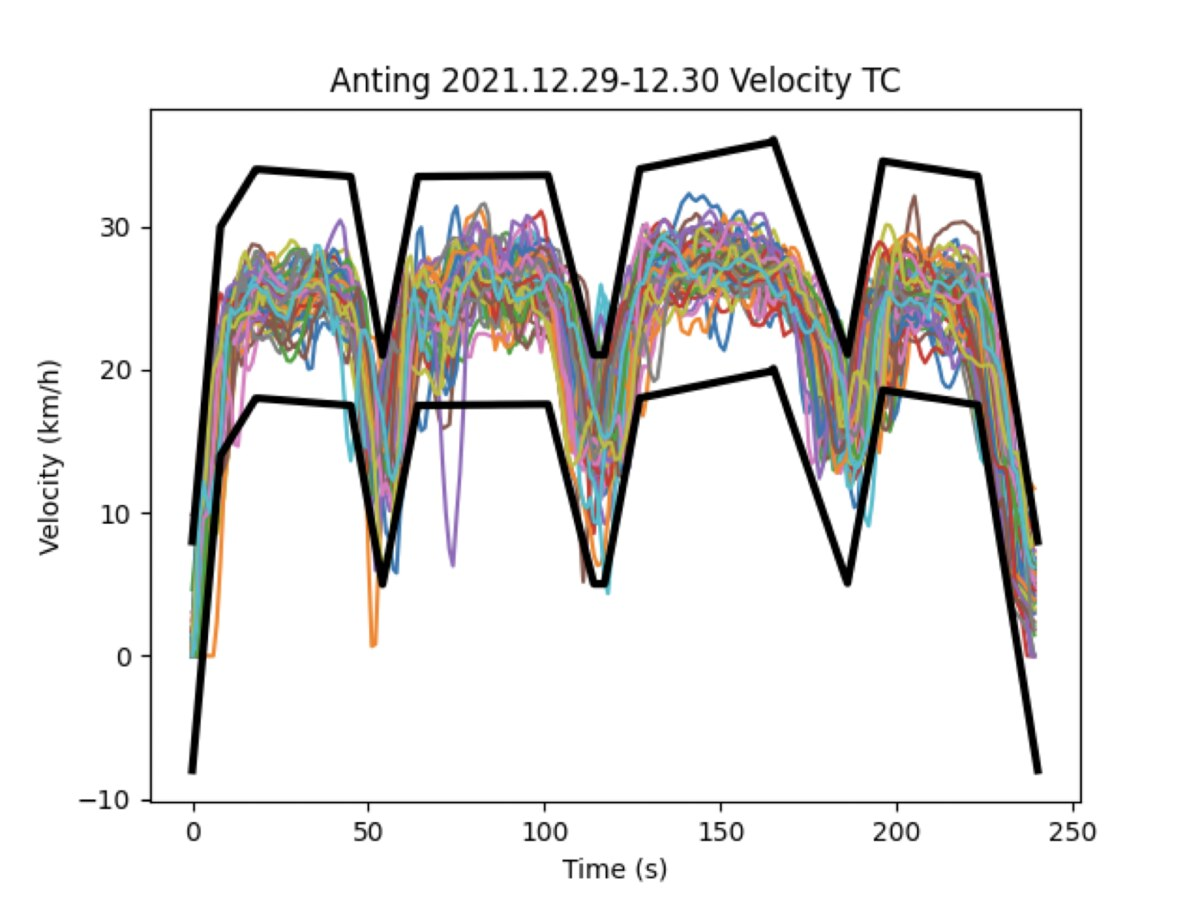
\includegraphics[width=0.82\textwidth]{images/optimized/openroad_b_velocity.jpg}
\end{center}
\end{column}
\begin{column}{0.44\columnwidth}
\begin{center}

\includegraphics[width=0.82\textwidth]{images/optimized/openroad_b_consumption.png}
\end{center}

\begin{itemize}
\item Frozen route-1 model
\item Different speed profile
\item About 4\% reduction without fine-tuning
\end{itemize}
\end{column}
\end{columns}
\end{frame}
\begin{frame}[label={sec:orgee77a4d}]{Multimodal road scenarios}
Traffic lights and pedestrians create multiple modes. The experiment
tags halt/non-halt states at three right turns, yielding eight modes.
\begin{columns}
\begin{column}{0.48\columnwidth}
\begin{center}

\includegraphics[width=0.82\textwidth]{images/optimized/openroad_mm_000_consumption.png}
\end{center}

Average reduction: 9.5\%
\end{column}
\begin{column}{0.48\columnwidth}
\begin{center}

\includegraphics[width=0.82\textwidth]{images/optimized/openroad_mm_111_consumption.png}
\end{center}

Average reduction: 4.3\%
\end{column}
\end{columns}
\end{frame}
\begin{frame}[label={sec:org82e9616}]{What the experiments show}
\begin{itemize}
\item Real reward-driven learning can be sample efficient when the MDP is
tightly scoped
\item Energy reduction emerges without hand-coded regenerative-braking rules
\item Frozen transfer works, but online adaptation gives stronger route
performance
\item Multimodal public-road behavior can be handled without manual scenario
policies
\item Driving-style drift must be measured, not assumed away
\end{itemize}
\end{frame}
\section*{Discussion}
\label{sec:org3eaf9bf}

\begin{frame}[label={sec:org5d1fb42}]{Deployment constraints}
Production deployment should include:

\begin{itemize}
\item Timestamped observations and bounded queues
\item Watchdog fallback to nominal pedal map
\item Stale-action rejection
\item Range-checked map updates
\item ECU or companion-processor latency budget
\item OTA validation before fleet rollout
\end{itemize}

\vspace{0.5em}

Cloud training is useful for fleet-scale updates; on-board inference is
preferred under strict latency requirements.
\end{frame}
\begin{frame}[label={sec:orge61a1df}]{Limitations and future work}
\begin{itemize}
\item Current observation window is too short for ramps and topographic
changes
\item Driving style is non-stationary over long windows
\item Recurrent policies can improve partial observability, but require more
data and memory
\item Offline RL can use uploaded fleet records for broader training
\item Diffusion policies may model multimodal behavior, but denoising steps
are challenging for real-time control
\end{itemize}
\end{frame}
\begin{frame}[label={sec:org911a39e}]{Takeaways}
\begin{enumerate}
\item EOSEV keeps the production driver-in-the-loop architecture.
\item The reward is measured electric work, not a fragile shaped proxy.
\item Bounded pedal-map updates create a practical action interface.
\item Real-road tests show about \(7\%\sim8\%\) weekly block-level reduction.
\item Scaling requires drift monitoring, transfer validation, and fleet-data
learning.
\end{enumerate}
\end{frame}
\end{document}
